\documentclass[12pt]{article}

\newcommand{\eqspace}{\hspace{1.5cm}} % Spacing between equations on same line
\def\Var{{\rm Var}\,} % Variance
\def\E{{\rm E}\,} % Expectation
\def\P{{\rm P}\,} % Probability

\usepackage{textcomp}
\usepackage{enumitem}
\usepackage{framed}
\usepackage{tablefootnote} % Allows command "\tablefootnote" for footnotes in tables
\usepackage{lastpage} % \pageref{LastPage} for last page number
\usepackage{wrapfig} % Allows "wrapfigure" environment

% To double-space
% \usepackage[doublespacing]{setspace}

\usepackage{apacite}

\usepackage{amsfonts}
\usepackage{amsmath} % More math symbols
\usepackage{amssymb} % More symbols
\usepackage{gensymb} % More symbols
%\usepackage{tipa} % IPA
%\usepackage{qtree} % Simple trees
\usepackage{amsthm} % Theorems
\usepackage{chemfig} % Chemical figures
\usepackage{chemmacros} % L and D chirality as \iupac{\L}
\usepackage[version=3]{mhchem} % Chemical figures
\usepackage{listings} % Pseudocode (examples in 15-451)

\usepackage{cleveref} % Allows \cref for smart references
\usepackage{graphicx}

\newtheorem{theorem}{Theorem} % Makes theorems work

% For drawing graphs
%\usepackage{tikz}
%\usetikzlibrary{arrows}

% For drawing Markov chains as per http://steventhornton.ca/markov-chains-in-latex/
%\usepackage{tikz}
%\usetikzlibrary{automata, positioning}

\usepackage{fancyhdr}

% header
\pagestyle{fancy}
\fancyhf{}
\lhead{ Cameron Wong (cjwong) \& Dylan Vrana (dtv) }
\chead{   }
\rhead{Page \thepage{} of \pageref{LastPage}}

\title{GPU Parallelization of the Li-Stephens Method for Genetic Imputation}
\author{Cameron Wong \& Dylan Vrana}

\begin{document}

\maketitle

\begin{abstract}

lol no generics

\end{abstract}

\section{Background}

Modern human genetics relies on two technologies for determining a person's genetic state.  The first is \textit{sequencing}, which measures a person's whole genome, totaling about 6 billion base pairs.  While complete, sequencing is expensive; even at scale, genome sequencing costs on the order of \$1000 per genome, though this is decreasing rapidly.  The other option is microarray genotyping in which, rather than measuring all base pairs in the human genome, a small subset of base pairs are selected for measurement.\footnote{Depending on application, this may be anything from 100 to 100,000.}  Most base pairs in the human genome are shared by all humans (and in fact shared with other species), making their measurement of little value.\footnote{There is still some value in measuring usually-constant base pairs- they can be modified by random (\textit{de novo}) mutations or by chromosomal abnormalities and deletions.}  Because genotyping is significantly less expensive than sequencing (about \$25 at scale) and can target only the subset of base pairs which vary within humans (referred to as \textit{Single Nucleotide Polymorphisms}, or \textit{SNPs}), it offers a low-cost alternative to sequencing which is, in most cases, sufficient for research and medical purposes.

However, a microarray cannot easily measure all SNPs.  A typical micrarray will measure 50k - 1M SNPs, while there are somewhere between 10M and 100M human SNPs, depending on what definitions are used.  Because measuring every SNP would become expensive (the very problem microarrays were designed to avoid), modern microarrays measure a subset of all SNPs and the remainder are \textit{imputed} (interred from existing data).  This is possible because of \textit{linkage disequilibrium}, the spatial intercorrelation of SNPs, which arises from biological properties of genetic recombination.

Most modern imputation algorithms are based on the Li-Stephens model, a first-order hidden Markov model that represents a genome as a series SNPs taken from reference \textit{haplotypes} (blocks of SNPs in close linkage disequilibrium) with a given \textit{jump probability} (probability of moving between haplotypes) \cite{listephens}. The majority of computation in Li-Stephens is involved in the \textit{forward-backward algorithm}, which calculates the posterior marginal probabilities of all possible hidden states given a sequence of observed emissions- here, the hidden states are ancestral genomes (represented by a reference panel) and the emissions are the known SNPs from which we are imputing.

\subsection{The Li-Stephens Model}

The model we present here (and implement) is a simplification of the full Li-Stephens model \cite{listephens}.  Our simplifications are purely to simplify some mathematics relevant to Li and Stephens' original goal of describing variation in recombination rate, but less relevant to our goal of imputation.  These changes do not alter the characteristics of the algorithmic problem.

We have $n$ sampled genomes $x_1 \ldots x_n$, each $T$ characters long.  These characters are taken from the alphabet $\Sigma = \{\text{A}, \text{T}, \text{C}, \text{G}\}$.  We also have a genome $y$ to be imputed, also $T$ characters long, where $O_t$ is the $t$th character emitted by $y$.  

Let $g$ be our garble rate (the probability that an observed SNP is mis-measured), $0 < g < 1$.  Let $\theta$ be a jump constant.  Let $d_t$ be the distance in map units\footnote{We use morgans, where one morgan is defined to be the distance along a chromosome over which one recombination event is expected.} between SNPs $t$ and $t+1$.

Then construct a hidden markov model of $n$ states, each one corresponding to a sampled genome.  Define a jump probability $J_t = 1 - e^{-d_t\theta}$.\footnote{Note that this means our transition probabilities depend on time step- technically not allowable in a Markov chain, but perfectly tractable for the algorithms we will use.}  The transition probability from state $i$ to state $j$ $\alpha_{ij}$ is

\[ a_{ij} = \begin{cases} 
      (1 - J_t) + \frac{J_t}{n} & i = j \\
      \frac{J_t}{n} & i \neq j \\
   \end{cases}
\]

The emission probability $e_t(z)$ is

\[ e_t(z) = \begin{cases} 
      1-g & z = O_t \\
      g & z \neq O_t \\
   \end{cases}
\]

\subsection{The Forward-Backward algorithm}

We are trying to discover $y_t$, the probability that the hidden state (here corresponding to the ``ancestral'' genome among our reference panel) at any given time $t$.  The Forward-Backward algorithm is a means of calculating the probability $P(y_t = x_t | O_{1:T})$ that a Markov process is in a given state at any time given an observed output sequence.  We do this via Bayes' rule

$$ P(x_t | O_{1:T}) = P(x_t | O_{1:O_t}, O{t+1:T}) \propto P(O{t+1:T} | x_t) P(x_t | O_{1:t}) $$

If we assume that the hidden state must be one of the $n$ hidden states we have (a necessary assumption for imputation), we can easily calculate the normalization factor by summing across all possible hidden states at time $t$.  We calculate $P(O{t+1:T} | x_t)$ via the backward algorithm and $P(x_t | O_{1:t})$ via the forward algorithm.  This means that the $P(O{t+1:T} | x_t)$ and $P(x_t | O_{1:t})$ we calculate must only be proportional to their real values across rows.  This will allow us to optimize our algorithm later.

\subsubsection{The Forward Algorithm}

The Forward algorithm is a dynamic algorithm for calculating $P(x_i | O_{1:t})$ given $n$ hidden states $x_1 \ldots x_n$ with transition probabilities $\alpha_{ij}$, emission probabilities $e_i(O_t)$, an observed sequence $O$, and an initial state $\pi$.  Take a matrix $A$ with $n$ columns and $T$ rows.  After running the algorithm, the $(t,i)$th element will be (proportional to) $P(x_i | O_{1:t})$.  

Initialize the first row to the initial state $\pi$.  Then, define every other cell by the recursive form

$$ A(t, i) = \sum_j \alpha_{ji} e_i(O_t) A(t-1, j) $$

This algorithm runs in $O(TN^2)$ work and $O(TN)$ span.  Its parallelism is limited by data dependencies- every cell in the $i+1$th row depends on every cell in the $i$th row.

\subsubsection{The Backward Algorithm}

The Backward algorithm is much like the Forward algorithm in structure.  It is a dynamic programming algorithm to calculate $P(O{t+1:T} | x_t)$.  While the Forward algorithm starts in the first row of the matrix and works forward in time, the Backward algorithm starts at the last row and works backwards in time.  Given the same inputs as the Forward algorithm, it initializes the last row to $e_i(O_T)$, then, defines every other cell by the recursive formula 

$$ B(t, i) = \sum_j \alpha_{ij} e_i(O_t) B(t+1, j) $$

This algorithm has the same runtime and general features as Forward.

\subsubsection{Smoothing}

Smoothing is a element-wise multiplication of the arrays $A$ and $B$.  We multiply such that 

$$ P(x_{it} | O_{1:T}) \propto A(t, i)B(t+1,i) $$

Then we normalize rows so all values sum to 1.  

This algorithm runs in $O(NT)$ work and $O(\log N)$ span.  

\section{Approach}

\subsection{Technologies Used}

We targeted NVIDIA GPU via CUDA.  We chose to target the GPU because running the Forward-Backward algorithm required a great deal of parallel floating point computation, well-suited for %TODO: this for Dylan

\subsection{Parallelizing Forward (and Backward)}

By taking advantage of natural characteristics of the Li-Stephens model, we are able to reduce the algorithm to $O(TN)$ work and $O(T\log N)$ span.

In the standard forward-backward algorithm, the forward and backward steps take the majority of the time; therefore, we will focus on them and disregard smoothing.  In addition, because the forward and backward algorithms have the same structure, I will describe a simplification of the forward algorithm that extends to the backward algorithm.

We perform the following reduction of the forward algorithm recurrence.

$$ A(t, i) = \sum_j \alpha_{ji} e_i(O_t) A(t-1, j) $$
$$ A(t, i) = e_i(O_t) (\sum_j \alpha_{ji}  A(t-1, j)) $$
$$ A(t, i) = e_i(O_t) ((1-J_t)A(t-1, j) + \sum_j \frac{J_t}{n} A(t-1, j)) $$
$$ A(t, i) = e_i(O_t) ((1-J_t)A(t-1, j) + \frac{J_t}{n}\sum_j A(t-1, j)) $$

Thus, for the Li-Stephens model, we can calculate the $i$th element relying on only the element immediately above it and the sum of the above row.  Summing a row takes $O(\log N)$ span, and computing the recursion can be parallelized, so computing the $i+1$th row from the $i$th row takes $O(\log N)$, and repeating this for the entire matrix takes $O(T\log N)$.\footnote{In practice, we normalize the above row (still takes $O(\log N)$) so that probabilities never get too small and we can avoid numerical issues.}

\subsection{Parallel Reduce}

In practice, however, a naive reduce is infeasible due to the width of the rows
being significantly larger than the maximum number of threads modern GPUs can
support (the Thousand Genomes Project, for example, contains around $N = 2500$
samples, over twice as many elements as the 1024 threads currently offered).
With a sufficiently large number of samples, we would break the reduce into
multiple recursive kernel invocations, and then reduce the chunked results.
We found this approach to be impractical. Instead, we found having each thread
compute the logarithmic sum of $\lceil\frac{N}{h}\rceil$ (where $h$ is the
maximum number of allowed threads) before doing a single-layered reduce on the
results to be sufficient. Modern genome sampling efforts only contain a low
multiple of $h = 1024$ samples, and so the recursive kernel was completely
dominated by kernel spawn overhead.

Of the micro-optimizations outlined in the NVIDIA developer
documentation \cite{reduceopt}, we were able to achieve speedup via address
interleaving (reducing divergent branching) and sequential addressing to reduce
shared bank conflicts, both of which gave significant speedup. We also
attempted to unroll the final warp as outlined (although we relied on compiler
pragmas over hand-unrolling), but found it to not provide much noticeable
speedup. Of particular note is that the optimizations intended to reduce
thread overhead by lowering the size of the block were not applicable to this
problem, as those threads are needed by the rest of the algorithm.

\newpage
\section{Results}

{
\begin{figure}[!hb]
  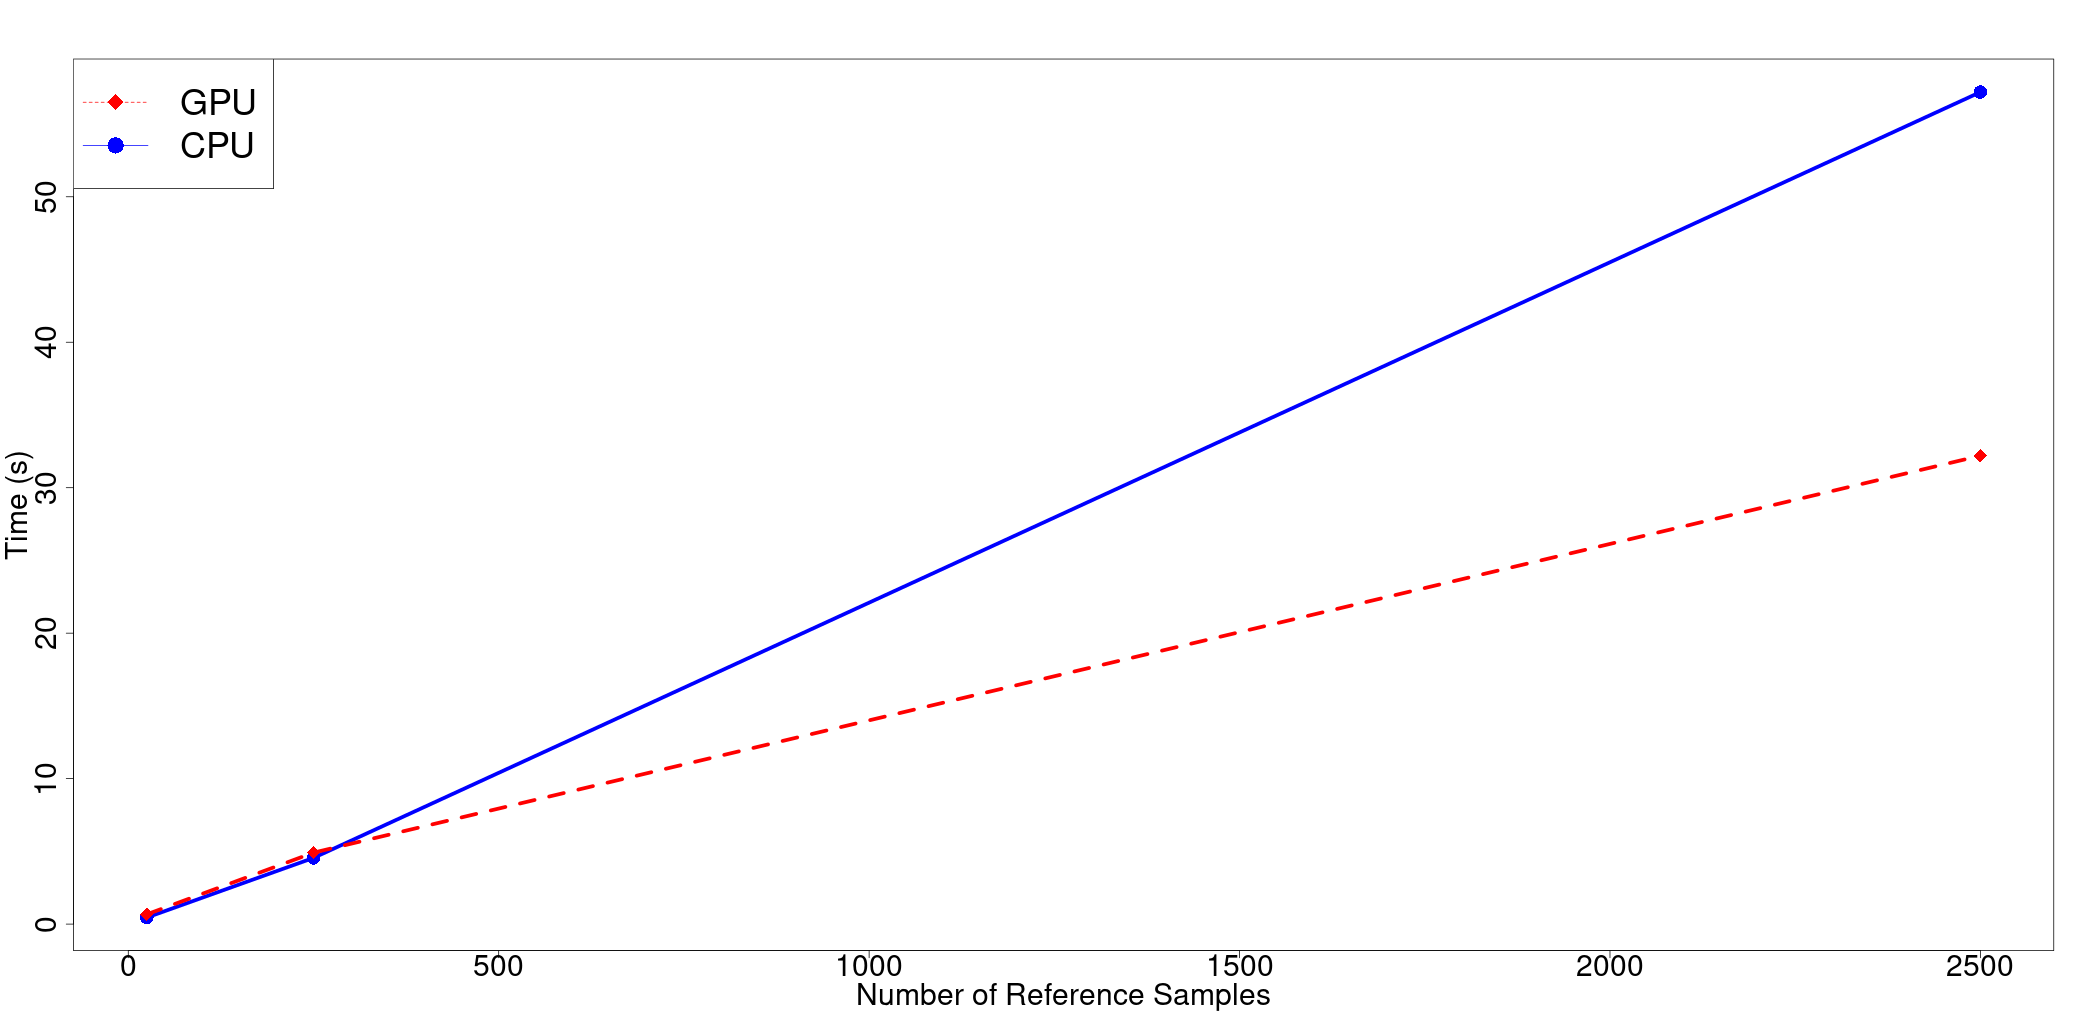
\includegraphics[scale=0.2]{sample}
\end{figure}
\begin{figure}[!hb]
  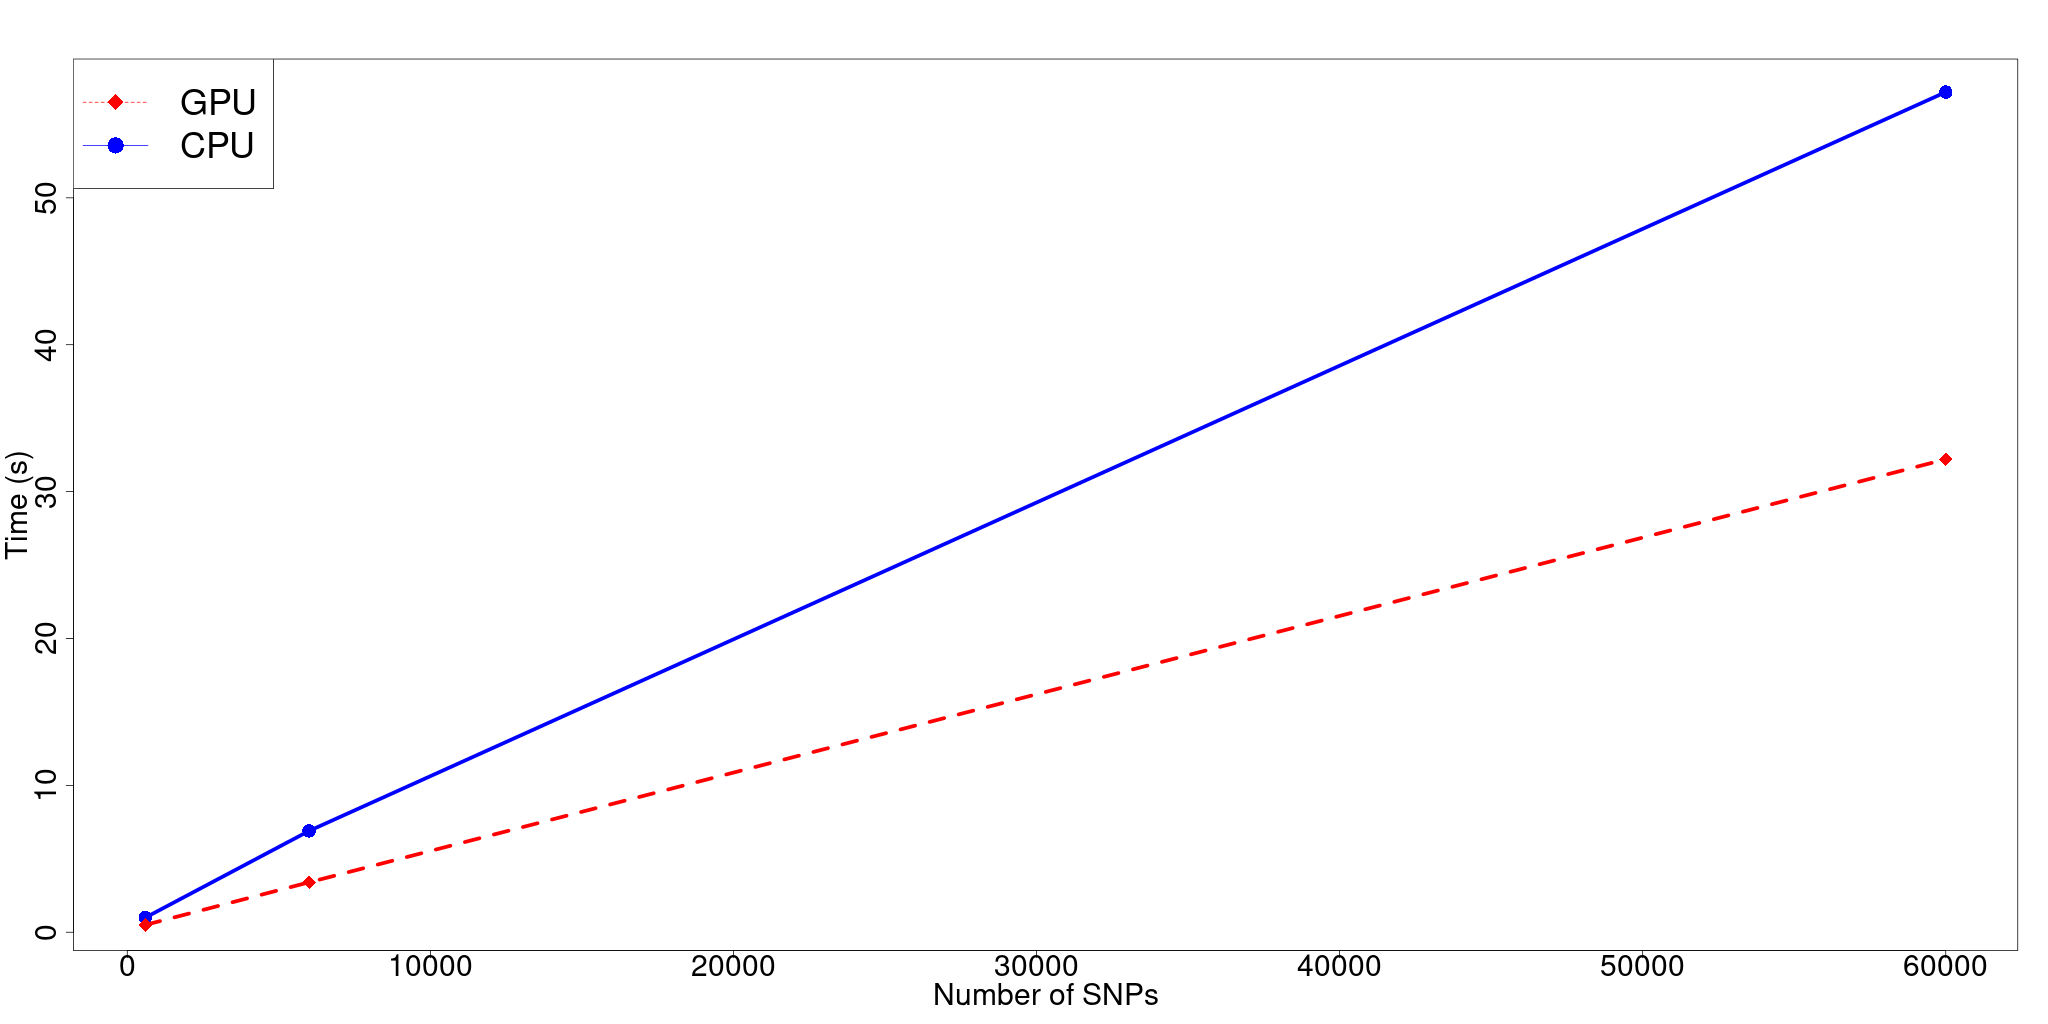
\includegraphics[scale=0.2]{snp}
\end{figure}
}

The blue line is a sequential LS algorithm executed on a single-core CPU, and
the red line is our parallel implementation performed on a single-core GPU.
These benchmarks were taken on the GHC machines, particularly GHC40.

Benchmarking was performed with $\theta = 1.0$ and $g = 0.1$ using randomly
generated test data, attempting to impute a single sample. This was done
because parallelizing over samples is trivial given multiple cores, as the
samples are simply imputed in a for loop (with no shared state between runs).

The two tables below are between two trials, as imputing one
person requires two runs. ``One trial'' consists of 1000 progrma runs with
times and speedups averaged.

% TODO: Dylan, look at this

% Also TODO: Cam, fix this formatting.

\begin{table}[ht]
  \caption{Data}
\begin{tabular}{l|lll|l}
Samples & SNPs  & GPU time (s) & CPU time (s) & Speedup       \\
        \hline
        & 600   & 0.19         & 0.01         & $\times 0.05$ \\
25      & 6000  & 0.22         & 0.06         & $\times 0.30$ \\
        & 60000 & 0.67         & 0.45         & $\times 0.67$ \\
        \hline
        & 600   & 0.22         & 0.10         & $\times 0.5$  \\
250     & 6000  & 0.60         & 0.63         & $\times 1.1$  \\
        & 60000 & 4.91         & 4.55         & $\times 0.92$ \\
        \hline
        & 600   & 0.51         & 1.02         & $\times 2$    \\
2500    & 6000  & 3.35         & 6.92         & $\times 2$    \\
        & 60000 & 32.2         & 57.2         & $\times 1.7$
\end{tabular}

\begin{tabular}{l|lll|l}
  Samples & SNPs & GPU time (s) & CPU time (s) & Speedup       \\
\hline
  & 600&0.0067       & 0.01         & $\times 1.5$  \\
  25 & 6000 &0.05         & 0.06         & $\times 1.13$ \\
  & 60000&0.49         & 0.45         & $\times 0.91$ \\
\hline
  & 600&0.05         & 1.01         & $\times 1.7$  \\
  250 & 6000&0.48         & 0.60         & $\times 1.2$  \\
  & 60000 &4.80         & 4.54         & $\times 0.95$ \\
\hline
  & 600&0.38         & 1.01         & $\times 3$    \\
  2500 &6000 &3.25         & 6.83         & $\times 2$    \\
  & 60000&32.1         & 57.2         & $\times 1.7$
\end{tabular}
\end{table}

We also recorded the following two trials with 250000 samples
(roughly the size of the UK Bio Bank, the largest current genetic sample)
and 200 SNPs.

\begin{table}[!ht]
  \begin{tabular}{ll|l}
    GPU time (s) & CPU time (s) & Speedup \\
    \hline
    0.42 & 38.3 & $\times 89$ \\
    0.33 & 42.9 & $\times 130$ \\
  \end{tabular}
\end{table}

\subsection{Discussion}

Ultimately, we found these results to be somewhat disappointing. According to
profiling data, our GPU workload was spent 80-95\% in synchronization costs
(synchronizing the rows of the computation grid in lockstep). and over 60\% of
the remaining overhead was in memory transfer. This can be particularly noted
in the first trial results, which also included some ``warming up'' costs due
to a mistake in our benchmarking setup (these trials were timed from
near-program startup rather than in a tight loop within the program).

We found that, at modern sampling numbers (on the order of 2500), there is
simply not enough work to be done per row for the problem to fit well onto a
GPU. Increasing the number of SNPs does not add any opportunity for
parallelism, as each row depends on the sum of the last row. Samples appear to
scale very well, but modern data simply does not have enough samples for this
to be feasible -- a 2500-wide row does not afford enough speedup to noticeably
offset the additional GPU overhead. We predict that a well-optimized CPU
implementation would be able to far outstrip the $\times 2$ figure
demonstrated, but have been unable to confirm this.

However, moving forward, we believe that our work will prove to be important.
Current projections predict sample sizes to increase by a factor of $\times
100$ within the next five years. We were able to impute single samples from
generated test cases at that scale in under 0.5 seconds with our GPU
implementation. We predict that we could bring this figure even lower with
another optimization pass (this time optimizing for memory streaming, as at
this scale, the GPUs internal memory limits become very prohibitive).

\section{Division of Work}

Equal work was performed by both members.

\bibliographystyle{apacite}
\bibliography{report}

\end{document}
